\section{Concurrent garbage collection}

As mentioned in the introduction, one of design goals of our collection scheme is to maintain \emph{low pause times}. This is particularly important in low-latency use cases like Tezos nodes, which store over 350 million objects yet must never block for more than a second. Looking back at the benchmark from \cref{app:mark-benchmark}, we can easily spot a problem: when there are 220,000 or more objects in the graph and a disk-based backend is used, the \texttt{mark} function alone can take longer than a second to execute. Combining this with the fact that we are stopping the world during collection, we are more than likely to break the latency constraint for Tezos nodes. Although we could try to shave a few more milliseconds of runtime off the \texttt{mark} function, the problem would creep up again for larger graphs. Instead, we must address the root of the problem: can we avoid stopping the world altogether?

\subsection{Motivation and terminology}

To better understand why stopping the world is usually needed in tracing garbage collection, let's look at the example from \cref{fig:lost-object}. Here, a collection cycle has already started--notice that some objects are already colored grey and black--but some new objects in dotted lines have been added to the heap concurrently, along with a new branch in the reference store which points to these objects. Since the marking algorithm has already examined all the roots and colored them grey at the beginning of the cycle, the newly created objects will remain white for the entire cycle, and will therefore be reclaimed while they are still reachable--this is known in literature as the \emph{lost object problem}.

\vspace{-.5em}
\begin{figure}[ht]
  \caption{An illustration of the \textit{lost object} problem during a collection cycle.}
  \label{fig:lost-object}

  \centering
  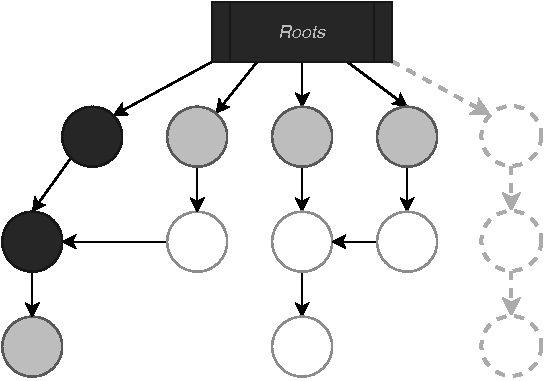
\includegraphics[width=0.4\textwidth]{images/lost-object.pdf}
\end{figure}


Attempts to solve this problem began with Steele~\cite{steele75}, Lamport~\cite{lamport76} and Dijkstra~\cite{dijkstra78}, giving birth to the field of \emph{concurrent garbage collection}. Note that the word concurrent is used in the strict sense here: without loss of generality, we will not consider whether we are trying to run the mutator and the collector in parallel--e.g. on multiple threads--or incrementally by interleaving their execution on a single thread. Instead, we will consider that the mutator and collector both operate in small, atomic operations; and simply look at the way these operations can be interleaved.

When mutator and collector operations become interleaved, the correctness of a garbage collection scheme is both a matter of \emph{safety}--the collector should preserve \emph{at least} all the reachable objects--and \emph{liveness}--every collection cycle should eventually complete. One way to reason about safety is to introduce the concept of \emph{wavefront}: in short, during the marking phase, the traversal can be seen as advancing a wavefront of grey objects, which separate the black objects from the white--unreached--objects. Note that, for the sake of simplicity, we consider here that the object graph contains a special object representing the mutator and pointing to all the mutator roots. Using this waveform abstraction, Wilson observes in~\cite{wilson94} that objects only become lost if the mutator stores a pointer to a white object inside a black object \emph{while} all paths from any grey objects to that white object are destroyed. This leads to the \emph{tricolor invariant}: in order for concurrent collection to be safe, no pointers to white objects must be added to black objects. Intuitively, this means that the collector must be able to assume that once objects become black, it won't need to look at them again during the rest of the cycle. \emph{Note that a weaker version of the tricolor invariant can be formulated, but is it not relevant in the context of this internship.}

Thanks to the special object introduced above, the eventuality of roots being updated during a collection cycle is also taken care of. Depending on the approach used for concurrent collection, this special object will either be given the color grey--meaning that the roots have either not been scanned or might need to be re-scanned--or the color black--meaning that the roots won't need to be scanned anymore.

\subsection{The special case of the Irmin heap}

Instead of digging through the classical techniques for concurrent collection, it is worth remembering that objects in the Irmin heap are immutable. This greatly simplifies the problem of maintaining the tricolor invariant, as concurrent collectors have to deal with the fact that black objects might mutate during a cycle, whereas the only object of the Irmin graph which can mutate during the cycle is the ``special object''--which corresponds to a change of roots, either because a branch was created, updated or deleted. With this in mind, I was able to come up with a relatively simple scheme for concurrent collection in Irmin. It uses a black mutator--meaning that the roots are only scanned once at the beginning of the collection cycle--and a \emph{write barrier}--meaning that the collector will hook into the \texttt{Store} and \texttt{Update} operations of the mutator to avoid breaking the tricolor invariant. \cref{app:concurrent-collection} is a pseudo-code implementation of this scheme.

In this scheme, the special mutator object becomes black at the beginning of the cycle--when \texttt{pending} is filled with \texttt{Roots()}--and stays black during the rest of the cycle. Therefore, to satisfy the tricolor invariant, every outgoing edge added to the mutator object during the cycle must point to a black or a grey object. If the target of that edge was stored during the cycle, it will already be black because of the \texttt{Store} hook, and otherwise it will be colored grey by the \texttt{Update} hook.

Notice that, while it might seem like the \texttt{Update} hook alone would be sufficient to maintain the invariant, the \texttt{Store} hook is needed too: what if an object were stored during a collection cycle, but the cycle finished before the user had time to create a branch referencing it?

Clearly, the time complexity of the marking phase remains unchanged, and the \texttt{Update} and \texttt{Store} hooks are each \(O(1)\). There is no such thing as a free lunch, however, and this concurrent scheme is no exception as it makes two trade-offs to avoid stopping the world. First, it sacrifices some promptness: objects which are stored during a collection cycle but never get referenced by a branch won't get reclaimed until the following cycle; nor will objects which were referenced by a branch at the start of a cycle but become unreachable because the branch gets deleted or updated during the cycle. Second, it can also add some memory overhead to the collection cycle since \texttt{Update} and \texttt{Store} can now add elements to \texttt{pending} and \texttt{marked}. This is usually acceptable, but might become a problem on single-threaded systems if the collector is interleaved with a lot of calls to \texttt{Store}, which might prevent the collector from doing any work while the size of \texttt{marked} grows unbounded.

Finally, astute readers may have noticed that this scheme only really solves part of the concurrency problem since tracing collection is a two-phase process, but we have only allowed concurrent execution of the mutator during the call to \texttt{mark}. To allow it during the entire cycle, we must also ensure that \texttt{backend.heap.Filter} plays nicely with the mutator. Since Irmin backends are modular by design, we don't have control over the concrete implementation of \texttt{Filter}; instead, we update the interface of backends, and require that a call to \texttt{Filter(p)} reclaims objects which do not pass \(p\) only if they have been stored into the backend \emph{before} the call to \texttt{filter}.

\subsection{Implementation details}

The complete implementation of concurrent garbage collection in Irmin is available in \cref{app:concurrent-modular-tracing}.

It is important to note that, in practise, the Irmin mutator and collector both run on the same thread--using the Lwt~\cite{lwt-manual} library for cooperative multitasking--so the execution of their operations is interleaved. First, this means that the problem of unbounded memory mentioned above might apply, so I've had to add a fail-safe which stops the collection cycle and clears \texttt{marked} and \texttt{pending} if their size grows significantly while the collector is unable to progress. Second, this puts us at the mercy of the Lwt scheduler: if the collector doesn't yield back to the scheduler enough; or if the scheduler groups the execution of collector operations without interleaving them with the mutator, the mutator will seem ``stopped'' for a few seconds to an outside observer--the very issue that we were trying to solve. This is particularly dangerous in the case of Tezos, which requires that the mutator always respond in less than a second. To alleviate the issue, I've had to adapt the signature of \texttt{cleanup} to let the caller specify a number of seconds or a number of processed objects after which the collector will be forced to yield back to the mutator, regardless of the scheduling policy of Lwt--as explained on \cref{lst:cleanup-sig}.

\vspace{-.8em}
\begin{figure}[ht]
  \caption{Signature of the \texttt{cleanup} function of Irmin databases.}
  \label{lst:cleanup-sig}

  \centering
  \vspace{-1em}
  \begin{minted}{ocaml}
val cleanup : ?roots:[ `Branches | `List of commit list ] ->
              ?limit_count:int -> ?limit_time:float -> t ->
              (unit, [> `Run_again ]) result Lwt.t
(** [cleanup t] runs the garbage collector on the object graph of database [t].
    Every commit, node and blob which is not reachable from [?roots] will be deleted.

    The garbage collector is concurrent, so collection can safely be interleaved with
    other database operations. This is done via two mechanisms:
    - the Lwt thread of the collector will yield on every I/O operation to allow other
      threads to execute while waiting for results;
    - the [?limit_count] and [?limit_time] options force the collector to return after
      processing more than a set number of objects or after running for a set number 
      of seconds. In this case, the function will return [Error `Run_again], and it
      will need to be run again at a later time to finish collection. *)
    \end{minted}
\end{figure}

\vspace{-1.5em}

As mentioned above, the interface of storage backends--specifically of \texttt{CONTENT\_ADDRESSABLE\_STORE}--must also be updated to mention the additional constraint on \texttt{filter}: a call to \mintinline{ocaml}{filter t p} now informs the content-addressable store that it can remove all values whose key \texttt{k} doesn't satisfy the predicate \texttt{p} \textit{only if they were present in the store before the call to} \texttt{filter}.

There are several ways for backends to handle this additional constraint. A trivial--but somewhat counterproductive--solution is to prevent the storage of new objects into the store during the call to \texttt{filter} altogether by using a lock. A somewhat better solution, which can be applied to every backend, is to allow new objects to be stored during the call to \texttt{filter} but keep track of the hashes of these objects using a set, so that objects get reclaimed only when they don't pass the predicate \emph{and} are not present in the set of recent objects. In some cases--e.g.~when the backend is a single pack-file--there even exist solutions without additional memory overhead; more on this in the chapter on \emph{Backend filtering strategies}.